% CMP 674 lesson presentation -- Hacettepe University, Computer Engineering.
% Theme: Hacettepe red + NVIDIA green.
% Build: `latexmk -pdf lesson.tex` (uses pdflatex; figures imported from
% ../paper/figures/).
\documentclass[10pt,aspectratio=169]{beamer}

% --- packages -----------------------------------------------------------------
\usepackage[utf8]{inputenc}
\usepackage[T1]{fontenc}
\usepackage{lmodern}
\usepackage{amsmath,amssymb}
\usepackage{graphicx}
\usepackage{booktabs}
\usepackage{multicol}
\usepackage{tikz}
\usetikzlibrary{positioning,arrows.meta,shapes,backgrounds,fit}
\usepackage{listings}
\usepackage{xcolor}

% --- color palette ------------------------------------------------------------
% Hacettepe red is the deep Bordeaux on the university's identity: a deep
% wine-red. NVIDIA green is the brand's #76B900.
\definecolor{HacettepeRed}{RGB}{168, 0, 43}
\definecolor{HacettepeRedDark}{RGB}{120, 0, 30}
\definecolor{HacettepeRedLight}{RGB}{220, 100, 130}
\definecolor{NvidiaGreen}{RGB}{118, 185, 0}
\definecolor{NvidiaGreenDark}{RGB}{75, 120, 0}
\definecolor{NvidiaGreenLight}{RGB}{200, 230, 130}
\definecolor{Charcoal}{RGB}{40, 40, 45}
\definecolor{LightGray}{RGB}{240, 240, 242}

% --- beamer theme -------------------------------------------------------------
\usetheme{default}
\useinnertheme{default}
\useoutertheme{default}

% Frame title style: red bar with white title text.
\setbeamercolor{frametitle}{fg=white,bg=HacettepeRed}
\setbeamercolor{title}{fg=HacettepeRed}
\setbeamercolor{author}{fg=Charcoal}
\setbeamercolor{institute}{fg=Charcoal}
\setbeamercolor{date}{fg=Charcoal}
\setbeamercolor{section in toc}{fg=HacettepeRed}
\setbeamercolor{subsection in toc}{fg=Charcoal}
\setbeamercolor{itemize item}{fg=NvidiaGreen}
\setbeamercolor{itemize subitem}{fg=NvidiaGreenDark}
\setbeamercolor{itemize subsubitem}{fg=NvidiaGreenDark}
\setbeamercolor{enumerate item}{fg=NvidiaGreen}
\setbeamercolor{block title}{fg=white,bg=HacettepeRed}
\setbeamercolor{block body}{fg=Charcoal,bg=LightGray}
\setbeamercolor{alerted text}{fg=NvidiaGreenDark}
\setbeamercolor{normal text}{fg=Charcoal}
\setbeamercolor{structure}{fg=HacettepeRed}
\setbeamercolor{footline}{fg=white,bg=HacettepeRedDark}

% Frametitle: keep it tight and prominent.
\setbeamertemplate{frametitle}{%
  \nointerlineskip%
  \begin{beamercolorbox}[wd=\paperwidth,sep=8pt,leftskip=12pt,rightskip=12pt]{frametitle}%
    \strut\insertframetitle\strut%
    \hfill%
    {\scriptsize\insertframenumber{} / \inserttotalframenumber}%
  \end{beamercolorbox}%
}

% Footline: red bar with course code on left, slide number on right.
\setbeamertemplate{footline}{%
  \begin{beamercolorbox}[wd=\paperwidth,ht=10pt,dp=4pt,leftskip=10pt,rightskip=10pt]{footline}%
    \tiny CMP~674 -- Parallel Computing with GPUs -- Hacettepe University%
    \hfill%
    Mixed-Precision Attention on RTX~5080%
  \end{beamercolorbox}%
}

\setbeamertemplate{navigation symbols}{}
\setbeamertemplate{itemize item}{\textcolor{NvidiaGreen}{\(\blacktriangleright\)}}
\setbeamertemplate{itemize subitem}{\textcolor{NvidiaGreenDark}{\(\blacktriangleright\)}}
\setbeamertemplate{enumerate item}{\textcolor{NvidiaGreen}{\arabic{enumi}.}}

% Code listing style.
\lstset{
  basicstyle=\ttfamily\scriptsize\color{Charcoal},
  keywordstyle=\color{HacettepeRed}\bfseries,
  commentstyle=\color{NvidiaGreenDark}\itshape,
  stringstyle=\color{NvidiaGreen},
  breaklines=true,
  columns=fullflexible,
  keepspaces=true,
  showstringspaces=false,
  frame=leftline,
  framerule=2pt,
  rulecolor=\color{HacettepeRed},
  xleftmargin=8pt,
}

% Block style overrides.
\setbeamertemplate{blocks}[default]
\setbeamercolor{block title alerted}{fg=white,bg=NvidiaGreenDark}
\setbeamercolor{block body alerted}{fg=Charcoal,bg=NvidiaGreenLight}
\setbeamercolor{block title example}{fg=white,bg=NvidiaGreen}
\setbeamercolor{block body example}{fg=Charcoal,bg=NvidiaGreenLight}

% --- title slide content ------------------------------------------------------
\title{\textbf{Mixed-Precision Attention on Consumer Blackwell}}
\subtitle{A Pareto Replication Study from FP32 to NVFP4 on the RTX~5080\\
\textcolor{NvidiaGreenDark}{Five hand-rolled CUDA kernels, one controlled ablation.}}
\author{\large CMP~674 Course Project}
\institute{Computer Engineering, Hacettepe University}
\date{Spring 2026}

% =============================================================================
\begin{document}

% --- title slide --------------------------------------------------------------
{
\setbeamertemplate{footline}{}
\begin{frame}[plain]
  \begin{tikzpicture}[remember picture,overlay]
    % Top red band
    \fill[HacettepeRed] (current page.north west) rectangle ([yshift=-1.6cm]current page.north east);
    % Bottom green strip
    \fill[NvidiaGreen] ([yshift=0.6cm]current page.south west) rectangle (current page.south east);
    % Course code top-left
    \node[white,anchor=north west,font=\small] at ([xshift=0.6cm,yshift=-0.5cm]current page.north west) {%
      \textbf{CMP~674} -- Parallel Computing with GPUs%
    };
    % Hacettepe label top-right
    \node[white,anchor=north east,font=\small] at ([xshift=-0.6cm,yshift=-0.5cm]current page.north east) {%
      Hacettepe University \textbar{} Computer Engineering%
    };
    % Title block
    \node[anchor=north,text width=0.85\paperwidth,align=center] at ([yshift=-3.0cm]current page.north) {%
      {\Huge\bfseries\color{HacettepeRed} Mixed-Precision Attention\\ on Consumer Blackwell}\\[8pt]
      {\Large\color{Charcoal} A Pareto Replication Study from FP32 to NVFP4 on the RTX~5080}\\[14pt]
      {\large\color{NvidiaGreenDark}\textit{Five hand-rolled CUDA kernels, one controlled ablation.}}%
    };
    % Bottom info
    \node[anchor=south west,text width=0.5\paperwidth,font=\small] at ([xshift=0.6cm,yshift=1.0cm]current page.south west) {%
      \textbf{Course project presentation}\\
      Spring 2026%
    };
    \node[anchor=south east,text width=0.45\paperwidth,align=right,font=\small] at ([xshift=-0.6cm,yshift=1.0cm]current page.south east) {%
      \texttt{github.com/canoztas/}\\
      \texttt{cmp674-attention-blackwell}%
    };
  \end{tikzpicture}
\end{frame}
}

% --- agenda -------------------------------------------------------------------
\begin{frame}{Agenda}
  \begin{enumerate}
    \item \textbf{The problem.} Why is attention slow? Why does it run out of
          memory?
    \item \textbf{The hardware.} What is consumer Blackwell? What is the
          RTX~5080? Where do Tensor Cores fit in?
    \item \textbf{The ladder.} Five hand-rolled kernels, V0 to V4, each
          changing one thing.
    \item \textbf{The findings.}
      \begin{itemize}
        \item Memory wall breaks at V2 ($17\times$ reduction).
        \item V3 closes half the SDPA latency gap with FP8.
        \item V4 \textbf{loses} to V3 by $\approx 30\%$ (the negative
              result).
      \end{itemize}
    \item \textbf{Why this matters.} What you should take away as a kernel
          developer or systems engineer.
  \end{enumerate}
\end{frame}

% =============================================================================
\section{Part 1: The Problem}

\begin{frame}{What is attention, in one slide}
  \begin{block}{The mechanism that made transformers possible}
    For each query $q_i$, look at every other token's key $k_j$, score the
    pair with $q_i \cdot k_j$, run a softmax over the scores, and use the
    resulting weights to mix the values $v_j$. Output is a weighted sum:
  \end{block}
  \[
    \mathrm{Attn}(Q, K, V) =
    \mathrm{softmax}\!\left(\tfrac{Q K^\top}{\sqrt{D}}\right) V.
  \]
  \begin{itemize}
    \item $Q, K, V$ are \textbf{$N \times D$} matrices (sequence length $N$,
          head dimension $D$).
    \item $Q K^\top$ is \textbf{$N \times N$} -- the score matrix.
    \item Softmax is row-wise; the result is the probability matrix $P$.
    \item $P V$ gives the output $O$, which is again $N \times D$.
  \end{itemize}
  \begin{alertblock}{Why this is the bottleneck}
    The score matrix $S = Q K^\top$ is \textbf{quadratic in $N$}. At
    sequence length 8{,}192 with batch 2 and 8 heads, that's
    $2 \cdot 8 \cdot 8192^2 \cdot \mathrm{sizeof(float)} \approx 4.3$~GB
    just for $S$. At 16{,}384 it's $17$~GB and the GPU runs out of memory.
  \end{alertblock}
\end{frame}

\begin{frame}{Why attention is hard on hardware}
  \textbf{Two problems, not one.}
  \vspace{0.4em}
  \begin{block}{Problem 1: memory bandwidth}
    The big tensors ($Q$, $K$, $V$, $S$, $P$, $O$) live in HBM. Reading them
    once costs $O(N^2)$ bytes of HBM traffic per forward pass. On consumer
    Blackwell, HBM bandwidth is $\approx 960$~GB/s; for $N = 8192$,
    head\_dim $128$, batch $2$, heads $8$, we move several GB through HBM
    \textit{just} for $S$ and $P$.
  \end{block}
  \begin{exampleblock}{Problem 2: compute throughput}
    The two matmuls ($Q K^\top$ and $P V$) dominate FLOPs. Tensor Cores
    accelerate them \textbf{only if} you feed them the right data layout
    and the right precision. FP32 ALU is $\sim 50\times$ slower than FP16
    Tensor Cores; FP16 Tensor Cores are $\sim 2\times$ slower than FP8;
    FP8 are $\sim 2\times$ slower than FP4.
  \end{exampleblock}
  \vspace{0.3em}
  \textbf{Two levers, then.} Avoid materializing $S$ and $P$ (memory) \emph{and}
  use the narrowest precision Tensor Cores you can (compute). Our paper
  measures both, in isolation.
\end{frame}

\begin{frame}{The ``naive'' implementation, what it costs}
  \begin{columns}[T]
    \column{0.55\textwidth}
      Three separate kernel launches, all FP32:
      \begin{enumerate}
        \item \textbf{$Q K^\top$ matmul} writes the $N{\times}N$ score
              matrix $S$ to HBM.
        \item \textbf{Row-wise softmax} reads $S$, writes the
              $N{\times}N$ probability matrix $P$ back to HBM.
        \item \textbf{$P V$ matmul} reads $P$, writes the output $O$ to HBM.
      \end{enumerate}
      \vspace{0.5em}
      \textbf{Numbers, $N = 2048$, head\_dim $= 128$, batch $= 2$, heads $= 8$:}
      \begin{itemize}
        \item HBM traffic per forward $\approx$ 1.0~GB
        \item FP32 ALU only -- no Tensor Cores
        \item Latency $\approx$ \textbf{4{,}500} ms on RTX~5080
        \item Memory $\approx$ \textbf{640} MB
      \end{itemize}
    \column{0.45\textwidth}
      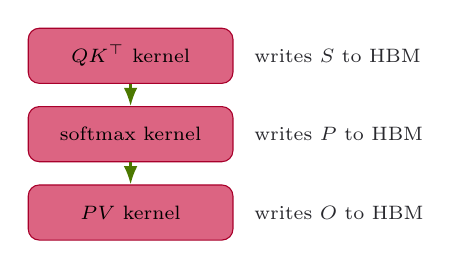
\begin{tikzpicture}[node distance=8pt,every node/.style={font=\scriptsize}]
        \node[draw=HacettepeRed,fill=HacettepeRedLight,rounded corners,
              minimum width=2.6cm,minimum height=0.7cm,text=black] (qk) {$Q K^\top$ kernel};
        \node[draw=HacettepeRed,fill=HacettepeRedLight,rounded corners,
              minimum width=2.6cm,minimum height=0.7cm,below=of qk,text=black] (sm) {softmax kernel};
        \node[draw=HacettepeRed,fill=HacettepeRedLight,rounded corners,
              minimum width=2.6cm,minimum height=0.7cm,below=of sm,text=black] (pv) {$P V$ kernel};
        \node[right=4pt of qk,text=Charcoal] {writes $S$ to HBM};
        \node[right=4pt of sm,text=Charcoal] {writes $P$ to HBM};
        \node[right=4pt of pv,text=Charcoal] {writes $O$ to HBM};
        \draw[-{Latex},thick,NvidiaGreenDark] (qk) -- (sm);
        \draw[-{Latex},thick,NvidiaGreenDark] (sm) -- (pv);
      \end{tikzpicture}
      \vspace{1em}
      \begin{alertblock}{What this is good for}
        Correctness baseline. Every other variant is checked against
        this kernel's output. \textbf{V0 is our oracle.}
      \end{alertblock}
  \end{columns}
\end{frame}

% =============================================================================
\section{Part 2: The Hardware}

\begin{frame}{Consumer Blackwell, in numbers}
  \begin{columns}[T]
    \column{0.55\textwidth}
      \begin{block}{NVIDIA GeForce RTX~5080 (our card)}
        \begin{itemize}
          \item Architecture: \textbf{Blackwell, sm\_120a}
          \item \textbf{84} streaming multiprocessors
          \item \textbf{16 GB} GDDR7, $\approx 960$~GB/s
          \item 5\textsuperscript{th}-gen Tensor Cores
          \item Native FP8 (E4M3 / E5M2) and FP4 (NVFP4)
          \item Released early 2025
        \end{itemize}
      \end{block}
    \column{0.45\textwidth}
      \begin{exampleblock}{Datacenter Blackwell (B100/B200) for context}
        \begin{itemize}
          \item Architecture: \textbf{sm\_100a}
          \item Has \textbf{TMA} (Tensor Memory Accelerator)
          \item Has hardware-microscaled NVFP4 with row-major SMEM access
          \item CUTLASS \texttt{77\_blackwell\_fmha} reference example
                works \emph{only} on sm\_100a / sm\_103a
        \end{itemize}
      \end{exampleblock}
      \vspace{0.4em}
      {\small Consumer Blackwell looks like a smaller datacenter Blackwell,
      but \textbf{some of the most useful features are missing}. This
      matters for our V3 / V4 design.}
  \end{columns}
\end{frame}

\begin{frame}{Tensor Cores, three precisions}
  Same instruction family (\texttt{mma.sync}), three precisions, three
  throughputs. The kernel asks for one explicitly via inline PTX or via
  the high-level \texttt{nvcuda::wmma} API.
  \vspace{0.6em}
  \begin{center}
  \begin{tabular}{l l l c c}
    \toprule
    \textbf{Precision} & \textbf{Mnemonic} & \textbf{Width} & \textbf{Used by} & \textbf{Theoretical $\times$ FP16} \\
    \midrule
    FP16 (E5M10) & \texttt{HMMA.16816.F32}        & $16{\times}8{\times}16$ & V1, V2 (\texttt{wmma}) & 1$\times$ \\
    FP8 (E4M3)   & \texttt{QMMA.16832.F32.E4M3.E4M3} & $16{\times}8{\times}32$ & V3 (inline PTX) & 2$\times$ \\
    FP4 (E2M1)   & \texttt{QMMA.16832.F32.E2M1.E2M1} & $16{\times}8{\times}32$ & V4 (inline PTX) & 4$\times$ \\
    \bottomrule
  \end{tabular}
  \end{center}
  \vspace{0.5em}
  \begin{itemize}
    \item \textbf{HMMA = ``Half MMA''} (FP16 inputs, FP32 accumulator).
    \item \textbf{QMMA = ``Quarter MMA''} on consumer Blackwell SASS;
          covers FP8 and FP4 with the precision encoded in the suffix.
    \item Each instruction uses a per-thread \emph{fragment} layout
          fixed in PTX; you load operands into registers and call the
          instruction.
    \item FP4 specifically requires \texttt{sm\_120a}, \emph{not} plain
          \texttt{sm\_120}.
  \end{itemize}
\end{frame}

\begin{frame}{What FP8 and FP4 can actually represent}
  \begin{columns}[T]
    \column{0.5\textwidth}
      \begin{block}{FP8 (E4M3)}
        \begin{itemize}
          \item 4 exponent bits, 3 mantissa bits
          \item Max representable magnitude: \textbf{448}
          \item $\sim 16$ representable positive values
          \item Reasonable for unscaled inputs around 1
        \end{itemize}
      \end{block}
    \column{0.5\textwidth}
      \begin{alertblock}{FP4 (E2M1)}
        \begin{itemize}
          \item 2 exponent bits, 1 mantissa bit
          \item Max representable magnitude: \textbf{6}
          \item $\sim 6$ representable positive values
          \item \textbf{Useless without per-block rescaling}
        \end{itemize}
      \end{alertblock}
  \end{columns}
  \vspace{0.6em}
  \begin{block}{Microscaling, in plain language}
    The values you actually want to multiply (rows of $Q$, blocks of $K$,
    elements of $P$) live on a much wider scale than FP8 / FP4 can hold.
    \textbf{So you don't store the values directly.} You divide each block
    by its own absolute-max, store the small-range result, and multiply by
    that scale factor when you read it back. The mma instruction can
    operate on FP4 values; the scales live in FP32 and apply at the
    accumulator.
  \end{block}
\end{frame}

% =============================================================================
\section{Part 3: The Five-Variant Ladder}

\begin{frame}{The ladder, one slide}
  \begin{center}
  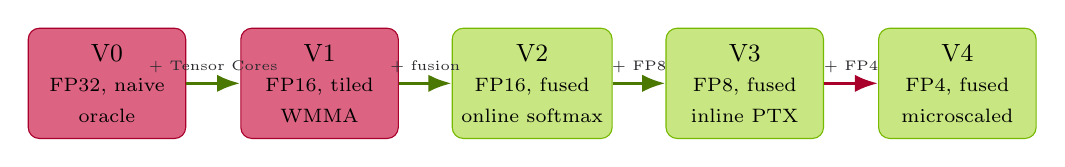
\begin{tikzpicture}[every node/.style={font=\small,align=center}]
    \node[draw=HacettepeRed,fill=HacettepeRedLight,rounded corners,minimum width=2.0cm,minimum height=1.4cm,text=black] (v0) at (0, 0) {V0\\\scriptsize FP32, naive\\\scriptsize oracle};
    \node[draw=HacettepeRed,fill=HacettepeRedLight,rounded corners,minimum width=2.0cm,minimum height=1.4cm,text=black] (v1) at (2.7, 0) {V1\\\scriptsize FP16, tiled\\\scriptsize WMMA};
    \node[draw=NvidiaGreen,fill=NvidiaGreenLight,rounded corners,minimum width=2.0cm,minimum height=1.4cm,text=black] (v2) at (5.4, 0) {V2\\\scriptsize FP16, fused\\\scriptsize online softmax};
    \node[draw=NvidiaGreen,fill=NvidiaGreenLight,rounded corners,minimum width=2.0cm,minimum height=1.4cm,text=black] (v3) at (8.1, 0) {V3\\\scriptsize FP8, fused\\\scriptsize inline PTX};
    \node[draw=NvidiaGreen,fill=NvidiaGreenLight,rounded corners,minimum width=2.0cm,minimum height=1.4cm,text=black] (v4) at (10.8, 0) {V4\\\scriptsize FP4, fused\\\scriptsize microscaled};
    \draw[-{Latex},very thick,NvidiaGreenDark] (v0) -- node[above,font=\tiny,Charcoal]{+ Tensor Cores}(v1);
    \draw[-{Latex},very thick,NvidiaGreenDark] (v1) -- node[above,font=\tiny,Charcoal]{+ fusion}(v2);
    \draw[-{Latex},very thick,NvidiaGreenDark] (v2) -- node[above,font=\tiny,Charcoal]{+ FP8}(v3);
    \draw[-{Latex},very thick,HacettepeRed] (v3) -- node[above,font=\tiny,Charcoal]{+ FP4}(v4);
  \end{tikzpicture}
  \end{center}
  \vspace{0.4em}
  \begin{block}{One change per step}
    The ladder is constructed so that each arrow changes \emph{exactly one}
    design choice. The performance and accuracy delta at each step
    therefore quantifies the contribution of that one choice on this
    hardware, with no confounding.
  \end{block}
  \vspace{0.4em}
  Spoiler: V0 to V3 are wins. V3 to V4 is a \textbf{loss}.
\end{frame}

\begin{frame}{V0: FP32 naive (the oracle)}
  \begin{columns}[T]
    \column{0.55\textwidth}
      \begin{itemize}
        \item Three separate kernel launches; full $S, P$ in HBM.
        \item \textbf{All FP32}: Tensor Cores not engaged at all.
        \item \textbf{Job:} pass the correctness test for every other
              variant. We check V1, V2, V3, V4 outputs against V0's output
              with relative-L2 tolerances.
        \item One \textbf{trap} we hit: the row-wise softmax reduction
              needs a \texttt{\_\_syncthreads()} between the two
              reduction phases. Without it: nondeterministic
              $\sim 6\%$ output mismatch on large $N$. Took several hours
              to find.
      \end{itemize}
    \column{0.45\textwidth}
      \begin{alertblock}{Numbers (\textit{N}=2048, \textit{D}=128)}
        \begin{itemize}
          \item Latency: \textbf{4{,}500} ms
          \item Memory: \textbf{640} MB
          \item Tensor Core insns: \textbf{0}
          \item Rel L2 vs FP32: \textbf{0} (it is the reference)
        \end{itemize}
      \end{alertblock}
      \begin{block}{What this teaches}
        Naive attention is unworkable past tiny $N$. \textbf{Optimization
        is not optional.}
      \end{block}
  \end{columns}
\end{frame}

\begin{frame}{V1: FP16 tiled, WMMA Tensor Cores}
  \begin{columns}[T]
    \column{0.6\textwidth}
      \begin{itemize}
        \item Same three-launch structure as V0, but inputs in FP16.
        \item Both matmuls go through the \texttt{nvcuda::wmma} API,
              which internally calls \texttt{HMMA.16816.F32}.
        \item \textbf{Trick \#1:} get $Q K^\top$ without an explicit
              transpose pass by loading $K$ as \texttt{matrix\_b
              col\_major}. Same memory, transposed in operand-space.
        \item \textbf{Trick \#2:} put all shared memory into a single
              dynamic allocation. Static + dynamic SMEM together count
              against a \textbf{48~KB} per-block default cap on Blackwell;
              we hit it exactly at $D = 128$.
        \item Still materializes $S$ and $P$ in HBM -- this is V2's
              problem to solve.
      \end{itemize}
    \column{0.4\textwidth}
      \begin{exampleblock}{Numbers (\textit{N}=8192, \textit{D}=128)}
        \begin{itemize}
          \item Latency: \textbf{77.1} ms
          \item Memory: \textbf{2176} MB
          \item HMMA insns: \textbf{120 + 32}
          \item Rel L2 vs FP32: $6 \times 10^{-4}$
        \end{itemize}
        \textit{$\approx 60\times$ faster than V0 already}, just from
        Tensor Cores. But still allocates 2~GB.
      \end{exampleblock}
  \end{columns}
\end{frame}

\begin{frame}{V2: FP16 fused -- the FlashAttention idea}
  \begin{block}{The big idea: \textbf{don't materialize $S$}}
    Process the keys and values in tiles, and combine the partial softmax
    results as you go. Maintain a running per-row \textbf{maximum} and a
    running \textbf{denominator}; rescale the partial output when a new
    maximum arrives.
  \end{block}
  \[
    \alpha^{(t)} = \exp(m^{(t-1)} - m^{(t)}),\quad
    O^{(t)} = \alpha^{(t)} O^{(t-1)} + \tilde P^{(t)} V^{(t)}.
  \]
  \begin{columns}[T]
    \column{0.55\textwidth}
      \begin{itemize}
        \item One fused kernel; one block per output row-tile.
        \item Per-block SMEM at $D = 128$ totals \textbf{96 KB}, over
              twice the default. Opt-in via\\
              \texttt{cudaFuncSetAttribute(...
              MaxDynamicSharedMemorySize, 96K)}.
        \item Two boundary cases not in the FA paper but \textbf{required}:
              first iteration ($m = -\infty$), fully-masked rows. Both
              produce NaN if you do the naive thing.
      \end{itemize}
    \column{0.45\textwidth}
      \begin{alertblock}{The 17$\times$ memory finding}
        At $N = 8192$, $D = 128$:\\
        \textbf{V1 = 2176 MB} $\to$ \textbf{V2 = 128 MB}.\\
        Same FP16 contract, no precision change. The full $N{\times}N$
        $S, P$ never appear in HBM.
      \end{alertblock}
  \end{columns}
\end{frame}

\begin{frame}{V3: FP8 fused with hand-rolled \texttt{mma.sync}}
  \begin{columns}[T]
    \column{0.6\textwidth}
      \begin{itemize}
        \item Replaces V2's FP16 \texttt{wmma} with the FP8 (E4M3)
              \texttt{m16n8k32} sync mma, called via \textbf{inline PTX}.
        \item Per-thread fragment layout is \textbf{fully specified} in
              the PTX ISA -- not implementation-defined like in WMMA.
        \item Therefore we can keep the \textbf{output accumulator in
              registers} across the K/V loop and apply the per-iteration
              scaling in registers. V2 had to round-trip through SMEM.
        \item Per-tile FP8 scaling for $Q$, $K$, $V$, and $P$. One scale
              per tile, broadcast cooperatively, applied at the
              accumulator after each mma.
        \item Why not CUTLASS? Its FMHA reference example
              (\texttt{77\_blackwell\_fmha}) is gated to \texttt{sm\_100a}
              / \texttt{sm\_103a} only. \textbf{No FMHA reference for
              consumer Blackwell.}
      \end{itemize}
    \column{0.4\textwidth}
      \begin{exampleblock}{Numbers (\textit{N}=8192, \textit{D}=128)}
        \begin{itemize}
          \item Latency: \textbf{25.8} ms ($2.4\times$ V2)
          \item Memory: \textbf{128} MB (same as V2)
          \item QMMA insns: \textbf{96}
          \item Rel L2 vs FP32: $5 \times 10^{-2}$
        \end{itemize}
      \end{exampleblock}
      \begin{block}{Lever pulled}
        FP8 mma + register-resident accumulator. Both come from the same
        change: \textit{the layout was knowable.}
      \end{block}
  \end{columns}
\end{frame}

\begin{frame}{V4: NVFP4 with software microscaling -- the negative result}
  \begin{columns}[T]
    \column{0.6\textwidth}
      \begin{itemize}
        \item Same kernel structure as V3, but FP4 (E2M1) instead of FP8.
        \item Uses \texttt{kind::f8f6f4.m16n8k32}; FP4 packed into the
              \emph{middle} 4 bits of each byte.
        \item Software microscaling: per-row, per-K-block (block size 32)
              FP32 scales, applied at the accumulator before each mma's
              accumulation.
        \item Each mma now does an extra $\approx 12$ register ops to
              apply scales. Across 96 mmas per (kv iter, thread), this
              is $\approx 1100$ ops/thread/iter \textbf{overhead}.
        \item Why not the \textbf{hardware} \texttt{mxf4nvf4.m16n8k64}?
              Its operand layout is \emph{scattered} per-thread,
              incompatible with our row-major SMEM idiom. Engaging it
              requires \texttt{ldmatrix}-style swizzled SMEM -- multi-
              week scope.
      \end{itemize}
    \column{0.4\textwidth}
      \begin{alertblock}{Numbers (\textit{N}=8192, \textit{D}=128)}
        \begin{itemize}
          \item Latency: \textbf{33.4} ms ($\mathbf{0.77 \times}$ V3,
                slower)
          \item Memory: \textbf{128} MB
          \item QMMA insns: \textbf{96}
          \item Rel L2 vs FP32: $0.21$
        \end{itemize}
      \end{alertblock}
      \begin{block}{Lever pulled \emph{against} us}
        Software microscaling overhead $>$ FP4 throughput advantage.
        \textbf{This is a finding, not a failure.}
      \end{block}
  \end{columns}
\end{frame}

% =============================================================================
\section{Part 4: Findings}

\begin{frame}{Finding 1 -- Memory wall breaks at V2}
  \begin{center}
    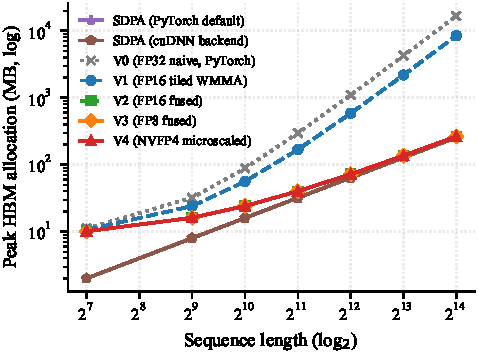
\includegraphics[width=0.62\linewidth]{../paper/figures/fig_memory_vs_seqlen.pdf}
  \end{center}
  \begin{itemize}
    \item V1 grows quadratically; V2 grows linearly.
    \item At $N = 8192$, $D = 128$: V1 = \textbf{2176 MB}, V2 = \textbf{128 MB}
          $\Rightarrow$ \textbf{17$\times$ reduction}.
    \item V2 / V3 / V4 / SDPA all overlap on this plot -- they all share
          the $O(N)$ profile.
    \item \textbf{This is what makes long-context inference possible on a
          16~GB consumer card.} Without it, $N = 16384$ at our
          $(\mathrm{batch}, \mathrm{heads})$ does not even fit.
  \end{itemize}
\end{frame}

\begin{frame}{Finding 2 -- V3 closes half the SDPA gap with FP8}
  \begin{columns}[T]
    \column{0.55\textwidth}
      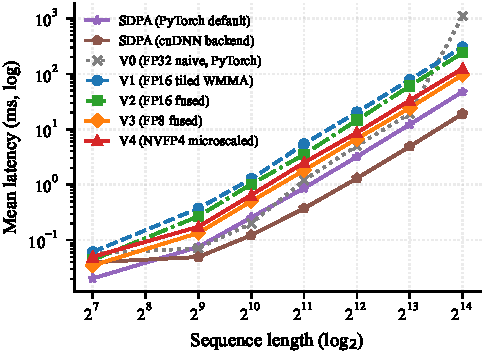
\includegraphics[width=\linewidth]{../paper/figures/fig_latency_vs_seqlen.pdf}
    \column{0.45\textwidth}
      At $N = 8192$, $D = 128$:
      \begin{itemize}
        \item V2: $\sim$60 ms
        \item V3: $\sim$26 ms (\textbf{2.4$\times$ V2})
        \item SDPA: $\sim$12 ms
      \end{itemize}
      \vspace{0.3em}
      \begin{alertblock}{Why V3 wins so much}
        \begin{itemize}
          \item FP8 mma throughput
            ($\sim 2\times$ FP16)
          \item Register-resident
            accumulator (V2 round-trips through SMEM)
        \end{itemize}
        Both come from the same change (PTX-specified fragment layout).
      \end{alertblock}
  \end{columns}
\end{frame}

\begin{frame}{Finding 3 -- V4 is \textbf{slower} than V3}
  \begin{center}
    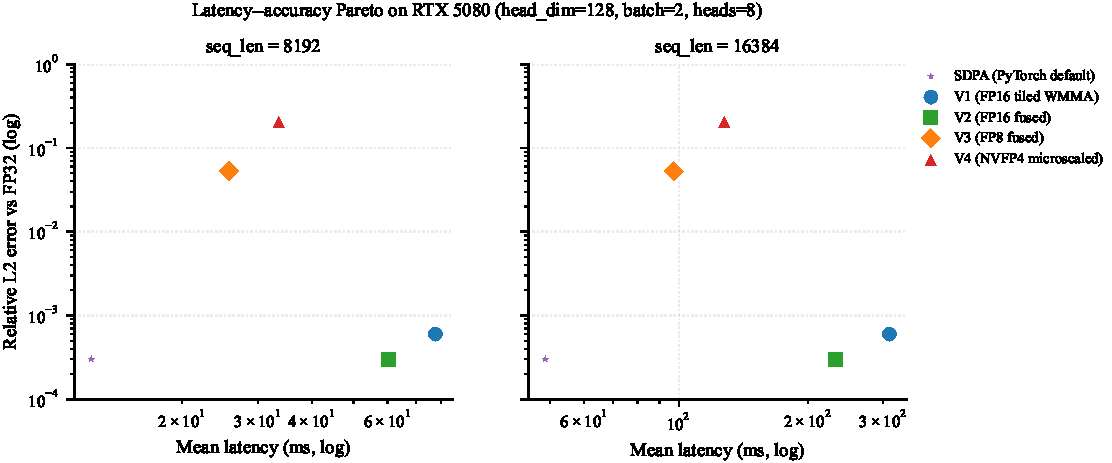
\includegraphics[width=0.6\linewidth]{../paper/figures/fig_pareto_main.pdf}
  \end{center}
  \begin{itemize}
    \item V4 (red triangle) sits at \textbf{higher latency} \emph{and}
          \textbf{higher error} than V3 (orange diamond). Dominated by V3.
    \item \textbf{The negative result.} On consumer Blackwell with our
          software-microscaled path, FP4's hardware throughput advantage
          (theoretical $2\times$ FP8) is more than canceled by the per-mma
          overhead.
    \item The hardware-microscaled \texttt{mxf4nvf4.m16n8k64} \emph{would}
          plausibly invert this. Its scattered-fragment layout is the
          blocker -- not the FP4 idea itself.
  \end{itemize}
\end{frame}

\begin{frame}[fragile]{Bonus finding: the SDPA dispatch is not what you think}
  \begin{block}{What we expected}
    PyTorch SDPA on the RTX~5080 dispatches to \textbf{FlashAttention-2 in
    FP16}. Beating it would mean beating a heavily-tuned FA-2 kernel.
  \end{block}
  \begin{alertblock}{What actually happens, in mid-2026, on Windows}
    The PyTorch~2.9.1+cu128 wheel was compiled \emph{without} flash
    attention. cuDNN attention and memory-efficient attention are also
    runtime-disabled for our (sm\_120, FP16, non-causal) inputs. SDPA
    \textbf{falls through to MATH backend} -- a pair of cuBLAS matmuls
    with a softmax in between.
  \end{alertblock}
  \vspace{0.3em}
  Concretely, when we tried to pin the dispatch:
  \begin{lstlisting}
with torch.nn.attention.sdpa_kernel(SDPBackend.FLASH_ATTENTION):
    F.scaled_dot_product_attention(Q, K, V)  # raises NoBackendError
  \end{lstlisting}
  \textbf{Methodological consequence:} comparing a custom kernel
  ``against SDPA'' without naming the dispatch can be misleading. Always
  pin the backend and disclose it.
\end{frame}

\begin{frame}[fragile]{Tensor Cores are actually engaged: \texttt{cuobjdump} proof}
  Nsight Compute's hardware counters require admin
  (\texttt{ERR\_NVGPUCTRPERM}). On a consumer card without admin we
  cannot use it. \textbf{So we read the SASS directly.}
  \vspace{0.5em}
  \begin{lstlisting}
cuobjdump --dump-sass kernels/v3_flash_fp8/_C.cp311-win_amd64.pyd `
    | Select-String QMMA | Measure-Object | % Count
# 96
  \end{lstlisting}
  \begin{center}
    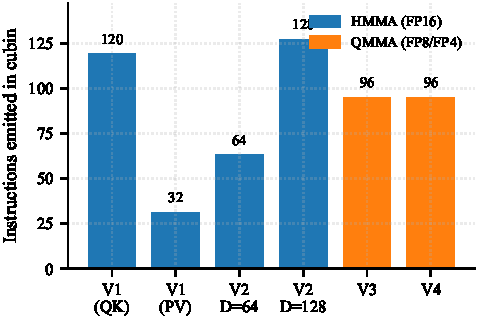
\includegraphics[width=0.62\linewidth]{../paper/figures/fig_tensor_core_engagement.pdf}
  \end{center}
\end{frame}

% =============================================================================
\section{Part 5: Why It Matters}

\begin{frame}{Pareto summary}
  \begin{center}
    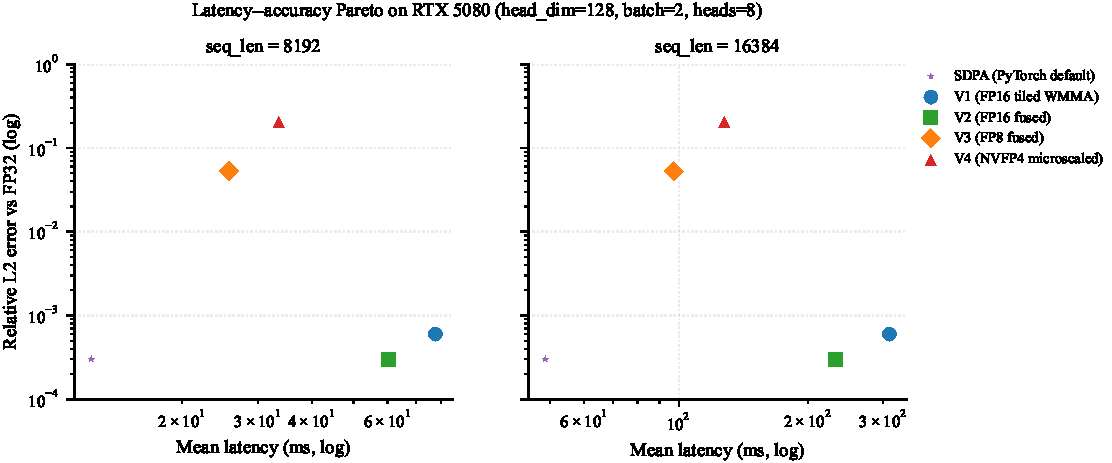
\includegraphics[width=0.85\linewidth]{../paper/figures/fig_pareto_main.pdf}
  \end{center}
  \begin{itemize}
    \item \textbf{V3 is the practical sweet spot} when you can absorb
          $\sim 5\%$ relative L2 error.
    \item SDPA is faster but has a hidden cost (it materializes $S$ and
          $P$; without flash, this is real HBM traffic).
    \item V4 sits dominated by V3 in this software stack.
  \end{itemize}
\end{frame}

\begin{frame}{What you should take away}
  \begin{enumerate}
    \item \textbf{Algorithmic fusion is the biggest single win.} The
          $17\times$ memory reduction at V1 $\to$ V2 came from changing
          the structure, not the precision.
    \item \textbf{Narrower precision pays off only when the layout is
          knowable.} The V2 $\to$ V3 latency win is half FP8 mma
          throughput, half register-resident O. Both require the
          fragment layout to be specified.
    \item \textbf{Lower precision is not strictly better.} FP4 lost on
          consumer Blackwell because the cheap-microscaling path is
          incompatible with the layouts we use elsewhere. Hardware
          quirks defeat ``obvious'' optimizations.
    \item \textbf{Vendor baselines are moving targets.} Pin your SDPA
          backend. State the build. Disclose the dispatch.
    \item \textbf{Read the SASS.} \texttt{cuobjdump} tells you exactly
          which Tensor-Core instructions you emitted. That is more
          reliable than runtime metrics gated by admin permissions.
  \end{enumerate}
\end{frame}

\begin{frame}{What I left undone (and why)}
  \begin{itemize}
    \item \textbf{Hardware-microscaled NVFP4
          (\texttt{mxf4nvf4.m16n8k64}).} Would likely flip V4 vs V3.
          Requires a swizzled SMEM layout incompatible with V3's idiom;
          multi-week scope on top of the existing kernel.
    \item \textbf{Backward pass.} Non-trivial for narrow-precision
          variants. The Attn-QAT paper documents specific instabilities;
          we focus on forward inference only.
    \item \textbf{RTX~5090 replication.} Same compute capability; very
          different SM count, memory bus, VRAM. Would tell us how much
          of the V4 result is hardware-microscaling-availability vs
          5080-specific.
    \item \textbf{Backend pinning that actually works.} The SDPA
          \texttt{FLASH\_ATTENTION} pin failed; on a Linux build with a
          flash-enabled wheel it would not. Re-running the comparison
          on Linux is a one-day item.
  \end{itemize}
\end{frame}

\begin{frame}[fragile]{Reproducibility -- it's two commands}
  \begin{lstlisting}
# Build the kernels (once per machine):
. .\env\activate_for_build.ps1
pip install --no-build-isolation -e kernels/v0_naive_fp32
pip install --no-build-isolation -e kernels/v1_tiled_fp16
pip install --no-build-isolation -e kernels/v2_flash_fp16
pip install --no-build-isolation -e kernels/v3_flash_fp8
pip install --no-build-isolation -e kernels/v4_flash_nvfp4

# Run the full sweep + figures:
python bench/run_all.py --config bench/configs/sweep_final.yaml `
    --output bench/results/sweep_final.parquet
python analysis/paper_figures.py
  \end{lstlisting}
  \vspace{0.5em}
  \begin{block}{What you get}
    \begin{itemize}
      \item One Parquet file with every per-iteration latency + provenance.
      \item Six figures and a LaTeX results table, regenerated from the
            Parquet.
      \item 495 passing pytest correctness tests across V0--V4.
    \end{itemize}
  \end{block}
\end{frame}

\begin{frame}{Q\,\&\,A}
  \begin{center}
    \vspace{1.5em}
    {\Huge\bfseries\color{HacettepeRed} Questions?}\\[1em]
    {\large\color{Charcoal} Code, paper, and slides:}\\[0.3em]
    \texttt{\large github.com/canoztas/cmp674-attention-blackwell}\\[2em]
    
\begin{tikzpicture}
      \fill[HacettepeRed] (0,0) rectangle (8,0.05);
      \fill[NvidiaGreen] (0,-0.15) rectangle (8,-0.10);
    \end{tikzpicture}\\[0.5em]
    {\small CMP~674 -- Parallel Computing with GPUs -- Hacettepe University}
  \end{center}
\end{frame}

\end{document}
